\documentclass[12pt,a4paper]{article}

\usepackage[utf8]{vietnam}
%\usepackage[tcvn]{vietnam}
\usepackage[T5]{fontenc}
\usepackage[utf8]{inputenc}
\usepackage[margin=2.5cm]{geometry}
\usepackage{amsmath}
\usepackage{amsfonts}
\usepackage{amssymb}
\usepackage{indentfirst}
\usepackage{rotating}
\usepackage{graphicx}
\usepackage{amsbsy}
\usepackage{epsfig}
\usepackage{natbib}
\usepackage{pdfpages}
\usepackage{multicol}
\usepackage{hyperref}
\usepackage{subfigure}
\usepackage{multimedia}
\usepackage{boxedminipage}
\usepackage{tikz}
\usepackage{nicefrac}
\usepackage{xcolor}
\usepackage{url}
\usepackage{listings}
\usepackage{color} % tô màu cho code
\usepackage{lipsum} %just for the example
\usepackage{listings}
\usepackage{enumerate}
%\usepackage[bottom]{footmisc}
%\fancyhf{}
\usepackage{tikz}
\newtheorem{proposition}{Mệnh đề}[section]
\newtheorem{theorem}{Định lý}[section]
\newtheorem{lemma}{Bổ đề}[section]
\newtheorem{corollary}{Hệ quả}[section]
\newtheorem{conjecture}{Dự đoán}[section]
\newtheorem{remark}{Chú ý}[section]
\newtheorem{example}{Ví dụ}
\newtheorem{problem}{Bài toán}[section]
\newtheorem{exercise}{Bài tập}
\newtheorem{define}{Định nghĩa}[section]
\usetikzlibrary{calc}


\makeatletter

\lstloadlanguages{C,C++,csh,Java}

\definecolor{red}{rgb}{0.6,0,0} 
\definecolor{blue}{rgb}{0,0,0.6}
\definecolor{green}{rgb}{0,0.8,0}
\definecolor{cyan}{rgb}{0.0,0.6,0.6}
 \definecolor{cloudwhite}{rgb}{0.9412, 0.9608, 0.8471}
\lstset{
language=csh,
basicstyle=\footnotesize\ttfamily,
numbers=left,
numberstyle=\tiny,
numbersep=5pt,
tabsize=2,
extendedchars=true,
breaklines=true,
frame=b,
stringstyle=\color{blue}\ttfamily,
showspaces=false,
showtabs=false,
xleftmargin=17pt,
framexleftmargin=17pt,
framexrightmargin=5pt,
framexbottommargin=4pt,
commentstyle=\color{green},
morecomment=[l]{//}, %use comment-line-style!
morecomment=[s]{/*}{*/}, %for multiline comments
showstringspaces=false,
morekeywords={ abstract, event, new, struct,
as, explicit, null, switch,
base, extern, object, this,
bool, false, operator, throw,
break, finally, out, true,
byte, fixed, override, try,
case, float, params, typeof,
catch, for, private, uint,
char, foreach, protected, ulong,
checked, goto, public, unchecked,
class, if, readonly, unsafe,
const, implicit, ref, ushort,
continue, in, return, using,
decimal, int, sbyte, virtual,
default, interface, sealed, volatile,
delegate, internal, short, void,
do, is, sizeof, while,
double, lock, stackalloc,
else, long, static,
enum, namespace, string},
keywordstyle=\color{cyan},
identifierstyle=\color{red},
backgroundcolor=\color{cloudwhite},
}

\usepackage{caption}
\DeclareCaptionFont{white}{\color{white}}
\DeclareCaptionFormat{listing}{\colorbox{blue}{\parbox{\textwidth}{\hspace{15pt}#1#2#3}}}
\captionsetup[lstlisting]{format=listing,labelfont=white,textfont=white, singlelinecheck=false, margin=0pt, font={bf,footnotesize}}



\begin{document}
\begin{titlepage}
\begin{tikzpicture}[remember picture,overlay,inner sep=0,outer sep=0]
     \draw[blue!70!black,line width=4pt] ([xshift=-1.5cm,yshift=-2cm]current page.north east) coordinate (A)--([xshift=1.5cm,yshift=-2cm]current page.north west) coordinate(B)--([xshift=1.5cm,yshift=2cm]current page.south west) coordinate (C)--([xshift=-1.5cm,yshift=2cm]current page.south east) coordinate(D)--cycle;

     \draw ([yshift=0.5cm,xshift=-0.5cm]A)-- ([yshift=0.5cm,xshift=0.5cm]B)--
     ([yshift=-0.5cm,xshift=0.5cm]B) --([yshift=-0.5cm,xshift=-0.5cm]B)--([yshift=0.5cm,xshift=-0.5cm]C)--([yshift=0.5cm,xshift=0.5cm]C)--([yshift=-0.5cm,xshift=0.5cm]C)-- ([yshift=-0.5cm,xshift=-0.5cm]D)--([yshift=0.5cm,xshift=-0.5cm]D)--([yshift=0.5cm,xshift=0.5cm]D)--([yshift=-0.5cm,xshift=0.5cm]A)--([yshift=-0.5cm,xshift=-0.5cm]A)--([yshift=0.5cm,xshift=-0.5cm]A);


     \draw ([yshift=-0.3cm,xshift=0.3cm]A)-- ([yshift=-0.3cm,xshift=-0.3cm]B)--
     ([yshift=0.3cm,xshift=-0.3cm]B) --([yshift=0.3cm,xshift=0.3cm]B)--([yshift=-0.3cm,xshift=0.3cm]C)--([yshift=-0.3cm,xshift=-0.3cm]C)--([yshift=0.3cm,xshift=-0.3cm]C)-- ([yshift=0.3cm,xshift=0.3cm]D)--([yshift=-0.3cm,xshift=0.3cm]D)--([yshift=-0.3cm,xshift=-0.3cm]D)--([yshift=0.3cm,xshift=-0.3cm]A)--([yshift=0.3cm,xshift=0.3cm]A)--([yshift=-0.3cm,xshift=0.3cm]A);
\end{tikzpicture}
\thispagestyle{empty}
	
	\begin{figure}[ht]
	   \minipage{0.76\textwidth}
			
\includegraphics[width=4cm]{logo_Hust.png}
			\label{EscudoUNAM}
	   \endminipage
	   \minipage{0.32\textwidth}
			
\includegraphics[height = 4.9cm ,width=4cm]{logo_Sami.png}
			\label{EscudoFC}
		\endminipage
	\end{figure}
	
	\begin{center}

	\LARGE
	TRƯỜNG ĐẠI HỌC BÁCH KHOA HÀ NỘI 
	

	\LARGE
	VIỆN TOÁN ỨNG DỤNG VÀ TIN HỌC
	
	\vspace{1cm}	
	\Large
	\textbf{BÁO CÁO CUỐI KỲ\\TÍNH TOÁN SONG SONG }

	\vspace{0.9cm}
	\normalsize	
	\large Giảng viên hướng dẫn \\
	\vspace{.3cm}
	\large
	\textbf{TS. Đoàn Duy Trung}
	
	\vspace{0.9cm}
	\normalsize	
	\large Nhóm báo cáo \\
	\vspace{.3cm}
	\large
	\textbf{Nhóm 05}
	
	\vspace{0.9cm}
	\normalsize	
	 \large Thành viên: \\
	 \end{center}

	\vspace{.3cm}
\begin{center}
	\begin{tabular}{lll}
		\Large 1.   &  \Large  Nguyễn Hữu Thuật & \Large 20185410\\
		\Large 2. & \Large Trần Xuân Hiếu  & \Large 20185354\\
		\Large 3.  & \Large Lại Tiến Long  & \Large 20185376 \\
		\Large 4.  & \Large Trang Hải Long  & \Large 20185382\\
		
	\end{tabular}	
\end{center}

\vspace{1.5cm}
\begin{center}
\large Hà Nội, Tháng 06 năm 2020
\end{center}
\end{titlepage}
	\newpage
%%===================================
\begin{center}
\textbf{\textbf{\Large  Lời cảm ơn}}
\end{center}	

Chúng Em xin gửi lời cảm ơn chân thành và sự tri ân sâu sắc đối với Thầy Đoàn Duy Trung - giảng viên học phần Tính toán song song đã vô cùng nhiệt tình giảng dạy Chúng Em trong suốt học kỳ qua, cũng như đã hướng dẫn đề tài này để Nhóm có thể hoàn thành tốt nhất bài báo cáo cũng như học phần này.\\

Trong quá trình học tập, báo cáo cũng như làm bài báo cáo khó tránh khỏi những sai sót, rất mong Thầy bỏ qua. Đồng thời cũng do trình độ lý luận cũng như kinh nghiệm thực tiễn còn hạn chế nên bài báo cáo không thể tránh khỏi những thiếu sót, Chúng Em rất mong nhận được ý kiến đóng góp Thầy để Chúng Em học thêm được  nhiều kinh nghiệm và sẽ hoàn thành tốt hơn các bài báo cáo sắp tới.\\

\textit{Chúng Em xin chân thành cảm ơn!}
%%====================================	
\newpage
%%====================================
\begin{center}
\textbf{\textbf{\Large Phân công công việc}}\\
\end{center}	
Việc đưa ra mục phân công công việc là tương đối, vì trước khi tiến hành viết chương trình, các thành viên nhóm đã cùng hội ý để: hiểu đề bài, đưa ra ý tưởng và thuật toán sơ bộ cho chương trình.\\
Dưới đây là phần phân công công việc của nhóm:


\begin{enumerate}[i)]
	\item \textbf{Nguyễn Hữu Thuật:}
	\begin{itemize}
		\item Phân công, tổng hợp công việc;
		\item Làm bài 1 (phần bài tập chung);
		\item Cùng viết chương trình bài tập riêng;
		\item Làm báo cáo.
	\end{itemize}
	\item \textbf{Trần Xuân Hiếu:}
	\begin{itemize}
		\item Cùng viết chương trình bài 2 (phần bài tập chung);
		\item Kiểm tra, chỉnh sửa chương trình bài tập riêng.
	\end{itemize}
	\item \textbf{Lại Tiến Long:}
	\begin{itemize}
		\item Cùng viết chương trình bài 2 (phần bài tập chung);
		\item Kiểm tra, chỉnh sửa chương trình bài tập 1 (phần bài tập chung);
		\item Chạy chương trình lấy kết quả báo cáo.
	\end{itemize}
	\item \textbf{Trang Hải Long:}
	\begin{itemize}
		\item Viết chính chương trình bài tập riêng;
		\item Kiểm tra, chỉnh sửa chương trình bài tập 2 (phần bài tập chung).
	\end{itemize}

\end{enumerate}


%%=====================================
\newpage
\tableofcontents
\newpage
%%=======================================
\section{Bài tập chung}
\underline{\textbf{Bài 1}} Liệt kê các số chính phương từ 1 đến n, với n nhập từ bàn phím. Phân chia đoạn [1; n] thành các đoạn để chạy trên các executor trong Lưới. \\[1cm]

\underline{Kết quả:}\\[0.3cm]
Hình 1: Kết quả chạy chương trình với 5 luồng tham gia, mỗi luồng xử lý tối đa 2 số
\begin{center}
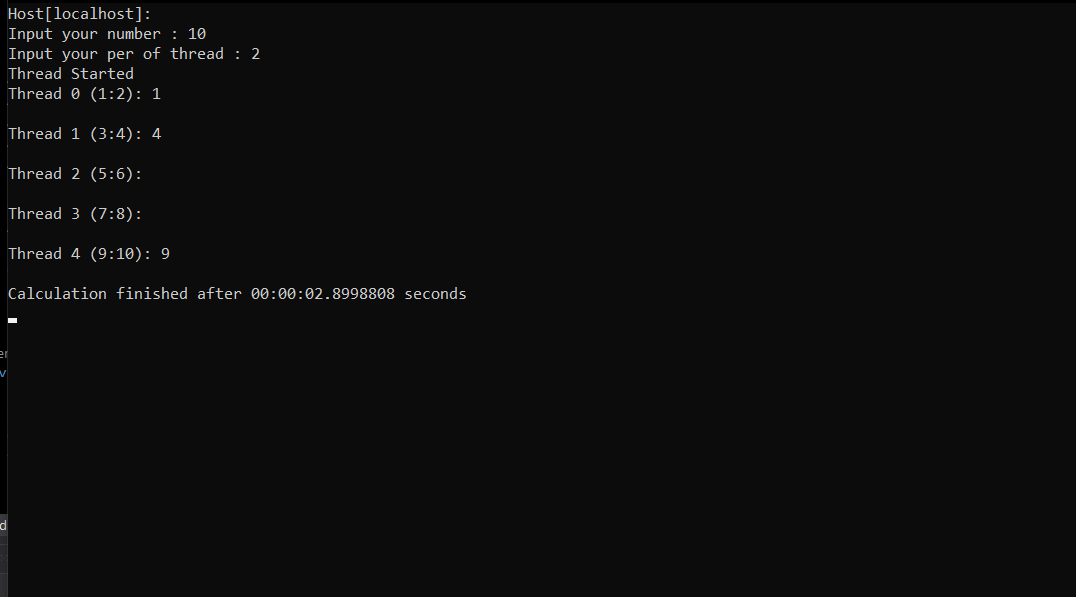
\includegraphics[scale=0.7]{2.png}\\[8cm]
\end{center} 



\underline{Alchemi Console:} \\[0.5cm]

Hình 2: 5 luồng đã được 2 Executor là DESKTOP-DDHDIOT và DESKTOP-TGSTI87 thực hiện
\begin{center}
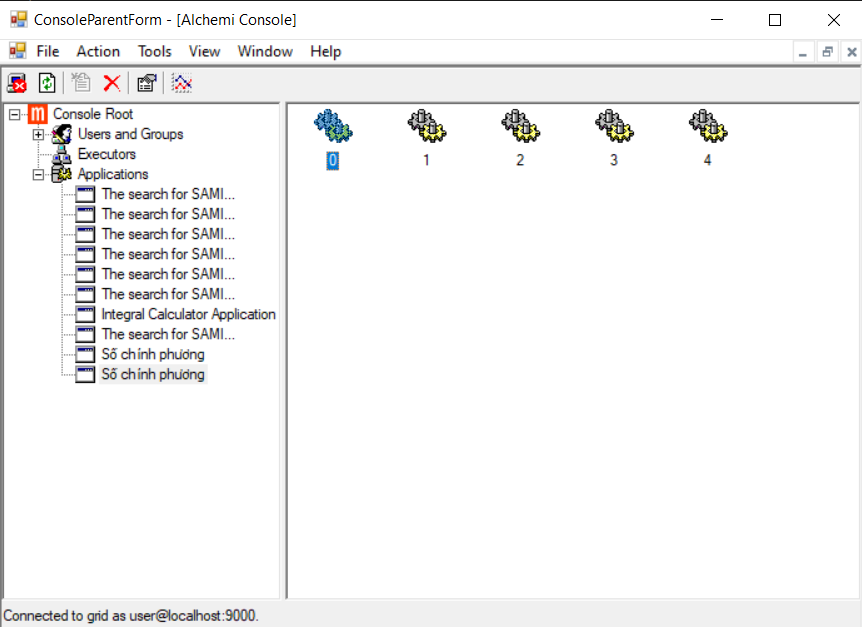
\includegraphics[scale=0.86]{2.0.png}
\end{center}



Hình 3: Luồng 0 do DESKTOP-TGSTI87 thực hiện
\begin{center}
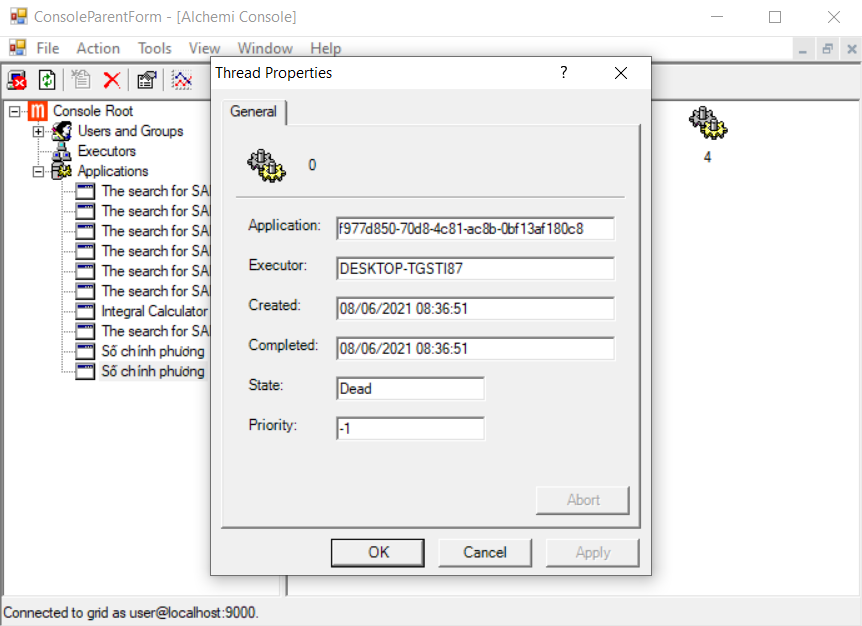
\includegraphics[scale=0.86]{2.1.png} \\[0.5cm]
\end{center}



Hình 4: Luồng 1 do DESKTOP-DDHDIOT thực hiện
\begin{center}
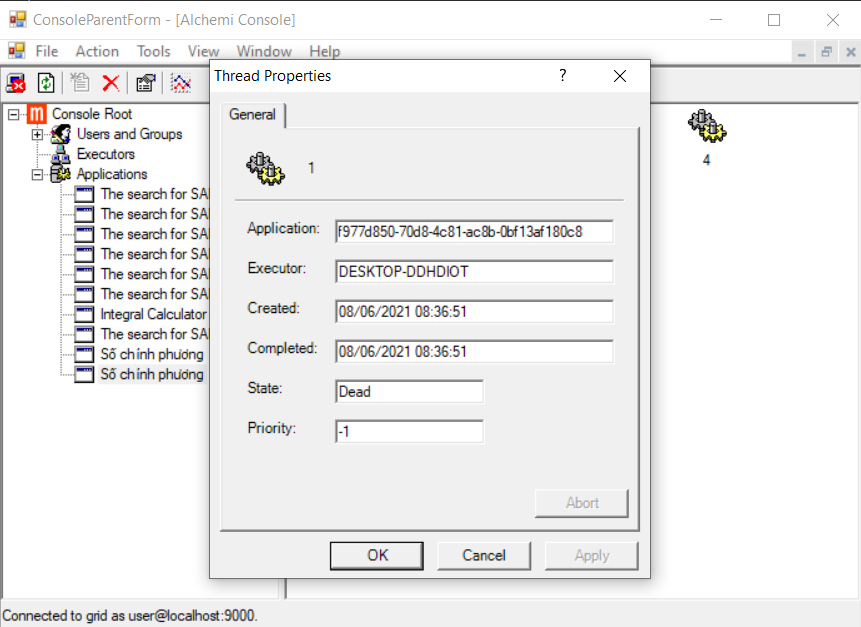
\includegraphics[scale=0.88]{2.2.png}
\end{center}

\newpage	

\underline{\textbf{Bài 2}}: Cho n nhập từ bàn phím. Tính gần đúng tích phân sau:
\begin{equation}
\displaystyle\int\limits_{0}^{n} f(x) \mathrm{d}x
\end{equation}
Ở đó hàm f(x) tùy ý;\\
Phân chia [0; n] vào các Executor để chạy trong Lưới. \\[1cm]

\underline{Kết quả:}\\[0.5cm]

Hình 5: Kết quả chạy chương trình với 10 luồng tham gia
\begin{center}
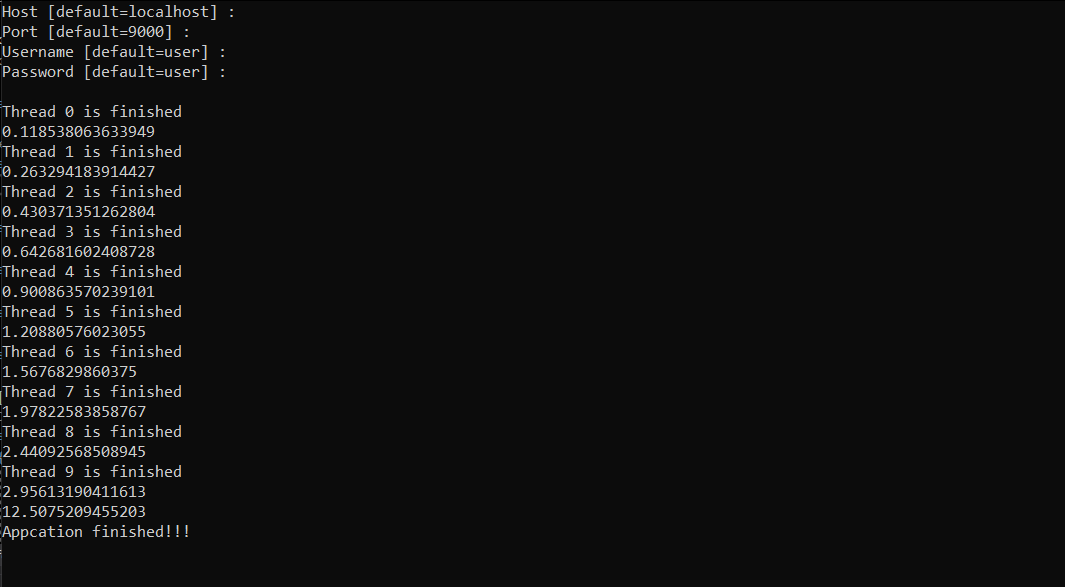
\includegraphics[scale=0.7]{3.png} \\[5.5cm]
\end{center}



\underline{Alchemi Console:}\\[0.5cm]

Hình 6: 10 luồng đã được 2 Executor là DESKTOP-DDHDIOT và DESKTOP-TGSTI87 thực hiện
\begin{center}
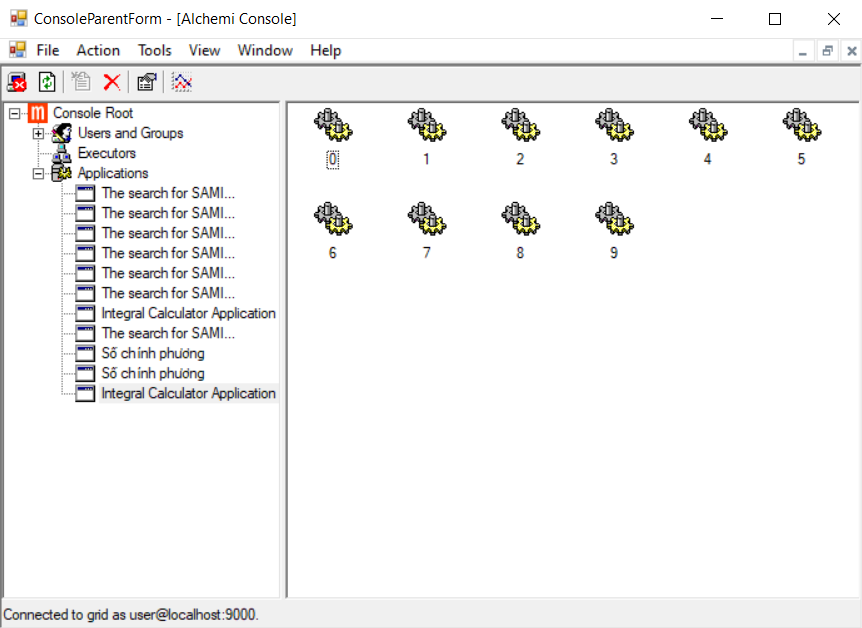
\includegraphics[scale=0.86]{3.0.png}
\end{center}



Hình 7: Luồng 0 do DESKTOP-TGSTI87 thực hiện
\begin{center}
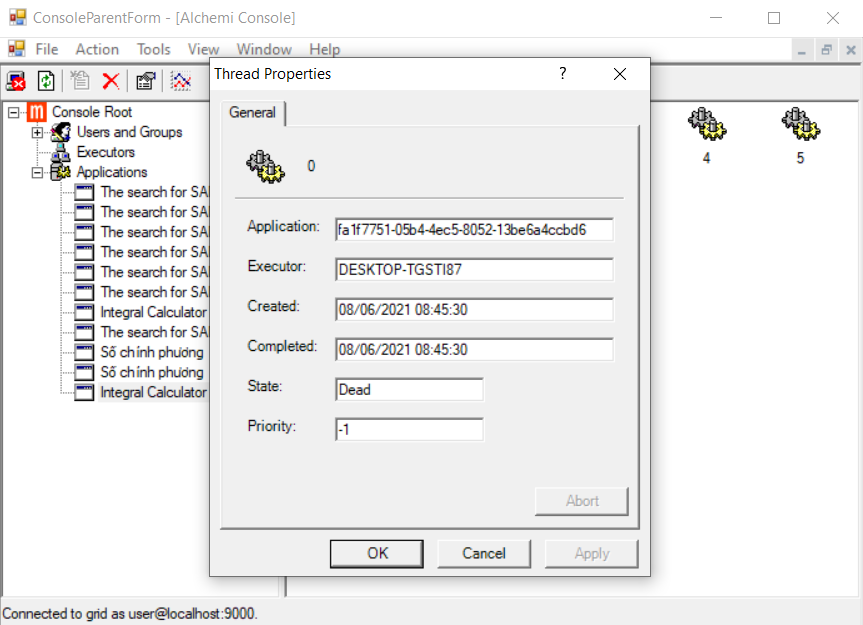
\includegraphics[scale=0.86]{3.1.png} \\[0.5cm]
\end{center}



Hình 8: Luồng 1 do DESKTOP-DDHDIOT thực hiện
\begin{center}
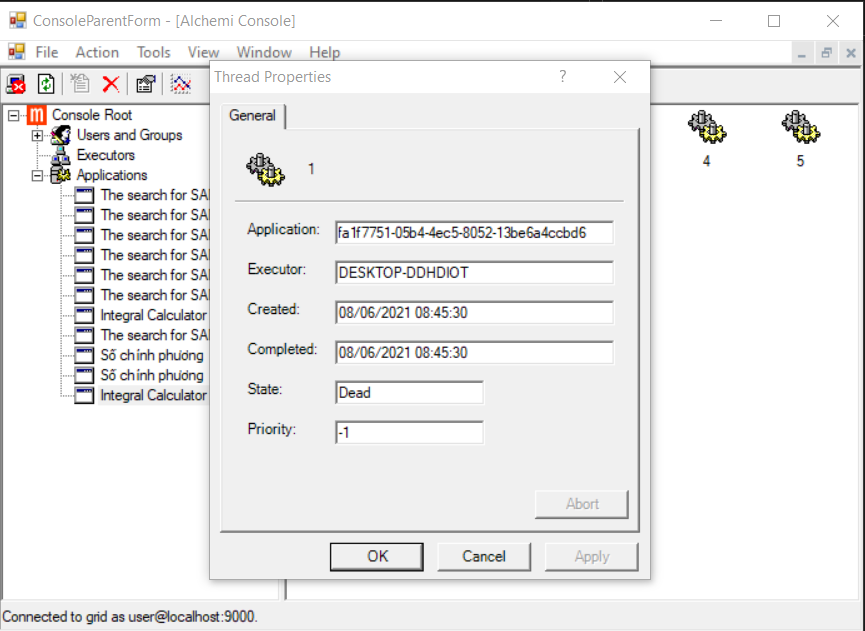
\includegraphics[scale=0.88]{3.2.png}
\end{center}



%%=====================================
\newpage

\section{Bài tập riêng}
\underline{\textbf{Đề 5}}: Đọc vào 1 đoạn văn bản dưới dạng file input.txt, tìm kiếm cụm từ SAMI xuất hiện đầu tiên trong 1 câu (1 câu kết thúc bởi dấu chấm). Phân chia văn bản thành nhiều k văn bản nhỏ hơn (k nhập từ bàn phím), mỗi văn bản nhỏ một vài câu. Yêu cầu mỗi văn bản nhỏ thực hiện trên 1 nút tính toán. Tổng hợp vị trí các cụm từ SAMI trên từng dòng vào file output.txt, nếu không có cum từ SAMI thì dòng đó để NULL. \\[0.5cm]

\subsection{Chương trình}
-----------------------------------------------------------------------------------------------------------------
\begin{lstlisting}
using System;
using System.Collections.Generic;
using Alchemi.Core.Owner;

namespace Parallel_Search_String
{
    class Program
    {
        static GApplication App;

        // Read the file as one string.
        static string text = System.IO.File.ReadAllText(@"..\..\document.txt");
        static List<string> sentences = new List<string>(text.Split('.'));
        static int NumberOfSentences = sentences.Count;
        static int SentencessPerThread = 2;
        static int NumThreads = 0;
            
        [STAThread]
        static void Main(string[] args)
        {
  			// Connect to Manager
            GConnection connection = GConnection.FromConsole("localhost", "9000", "user", "user");

       		// Create an application object that represents the application you are running
            App = new GApplication(connection); // Initialization
            App.ApplicationName = "The search for SAMI...";   // Assign the name of the application, this name will be displayed in the Alchemi Console window
            App.Manifest.Add(new ModuleDependency(typeof(StringSearchGridThread).Module));   

           // Always the number of calculations to use
            NumThreads = (Int32)Math.Floor((double)NumberOfSentences / SentencessPerThread);
            if (SentencessPerThread * NumThreads < NumberOfSentences)
            {
                NumThreads++;
            }

          // Create and add streams
            for (int i = 0; i < NumThreads; i++)
            {
                int StartIndex = i * SentencessPerThread;
                int SentencesForThisThread = Math.Min(SentencessPerThread, NumberOfSentences - i * SentencessPerThread);

StringSearchGridThread thread = new StringSearchGridThread(sentences.GetRange(StartIndex, SentencesForThisThread)); 
                App.Threads.Add(thread);   // Add thread to the application
            }

          // Events
            App.ThreadFinish += new GThreadFinish(OnThreadFinish);

           // App starts running
            App.Start();

            Console.ReadLine();
        }

     // Event to end a thread
        static public void OnThreadFinish(GThread th)
        {
            Console.WriteLine("Thread {0} finished the job", th.Id);
            StringSearchGridThread thread = (StringSearchGridThread)th;
            foreach (int i in thread.Result)
            {
                if (i == -1)
                {
                    Console.WriteLine("NULL");
                }
                else
                {
                    Console.WriteLine(i);
                }
            }
        }
    }
    [Serializable]
    class StringSearchGridThread : GThread
    {

        private List<int> _Result = new List<int>();
        private int _StartIndex;
        private int _NumSentences;
        private List<string> _Sentences = new List<string>();

		// Decorator
        public List<int> Result
        {
            get
            {
                return _Result;
            }
        }

        public List<string> Sentences
        {
            get
            {
                return _Sentences;
            }
        }
        public int StartIndex
        {
            get
            {
                return _StartIndex;
            }
        }

        public int NumSentences
        {
            get
            {
                return _NumSentences;
            }
        }

        // Constructor
        public StringSearchGridThread(List<string> Sentences)
        {
            _Sentences = Sentences;
        }
        public override void Start()
        {
            for (int i = 0; i < _Sentences.Count; i++)
            {
                _Result.Add(_Sentences[i].IndexOf("SAMI", 0));
            }
        }
    }
} 
\end{lstlisting}

\underline{\textbf{File Document.txt}} \\[0.5cm]
---------------------------------------------------------------------------------------------------------------------
\begin{lstlisting}
Institute of Applied Mathematics and Informatics (SAMI), Hanoi University of Science and Technology, is a prestigious undergraduate and graduate research and training institution in the field of Mathematics and Informatics. SAMI... The Institute's main tasks are: Teaching and researching mathematics, applied mathematics and informatics; Conduct research and teaching cooperation with domestic and foreign training institutions; Coordinating with branches, levels and enterprises in applying mathematics and informatics in fields such as economics, finance, construction, engineering, etc.SAMI.Institute of Applied Mathematics and Informatics (SAMI), Hanoi University of Science and Technology, is a prestigious undergraduate and graduate research and training institution in the field of Mathematics and Informatics. SAMI... The Institute's main tasks are: Teaching and researching mathematics, applied mathematics and informatics; Conduct research and teaching cooperation with domestic and foreign training institutions; Coordinating with branches, levels and enterprises in applying mathematics and informatics in fields such as economics, finance, construction, engineering, etc.SAMI.Institute of Applied Mathematics and Informatics (SAMI), Hanoi University of Science and Technology, is a prestigious undergraduate and graduate research and training institution in the field of Mathematics and Informatics. SAMI... The Institute's main tasks are: Teaching and researching mathematics, applied mathematics and informatics; Conduct research and teaching cooperation with domestic and foreign training institutions; Coordinating with branches, levels and enterprises in applying mathematics and informatics in fields such as economics, finance, construction, engineering, etc.SAMI.
\end{lstlisting}

\subsection{Kết quả}

Hình 9: Kết quả chạy chương trình với 10 luồng tham gia, mỗi luồng xử lý tối đa 2 câu
\begin{center}
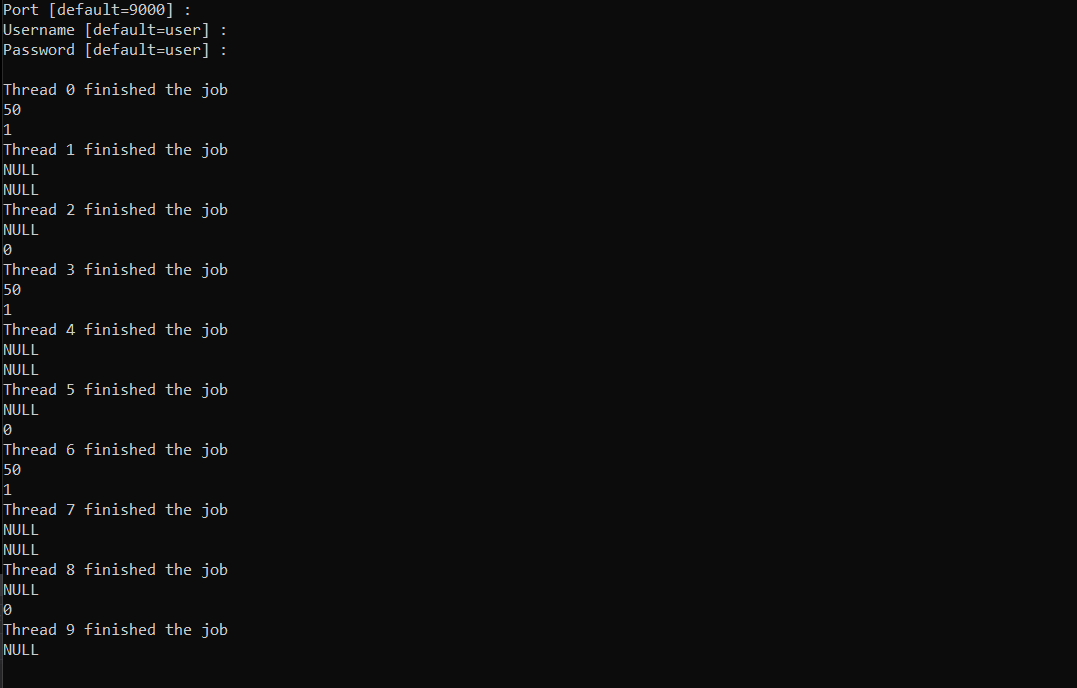
\includegraphics[scale=0.7]{1.2.png}
\end{center}




\subsection{Alchemi Console} 

Hinh 10: 10 luồng đã được 2 Executor là DESKTOP-DDHDIOT và DESKTOP-TGSTI87 thực hiện
\begin{center}
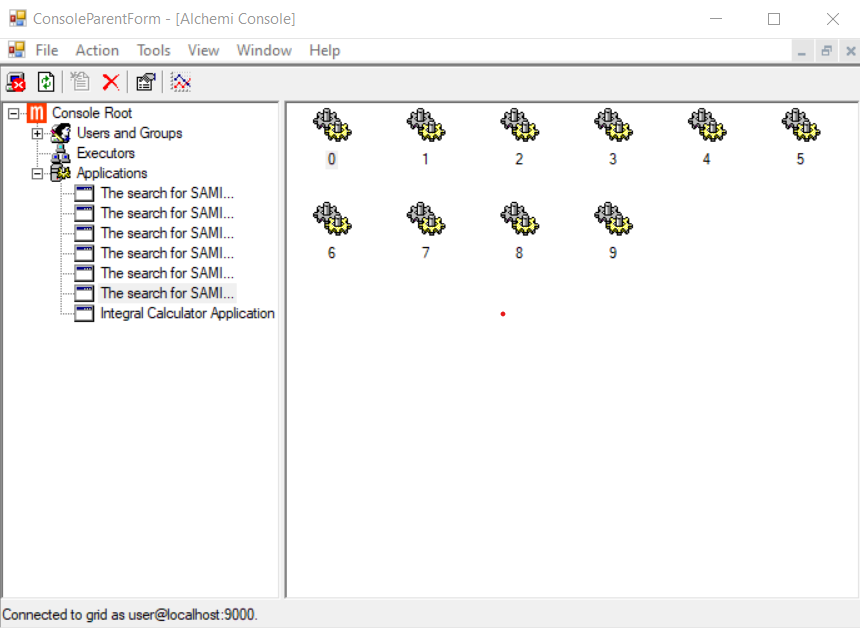
\includegraphics[scale=0.88]{1..png}
\end{center}



Hình 11: Luồng 0 do DESKTOP-DDHDIOT thực hiện
\begin{center}
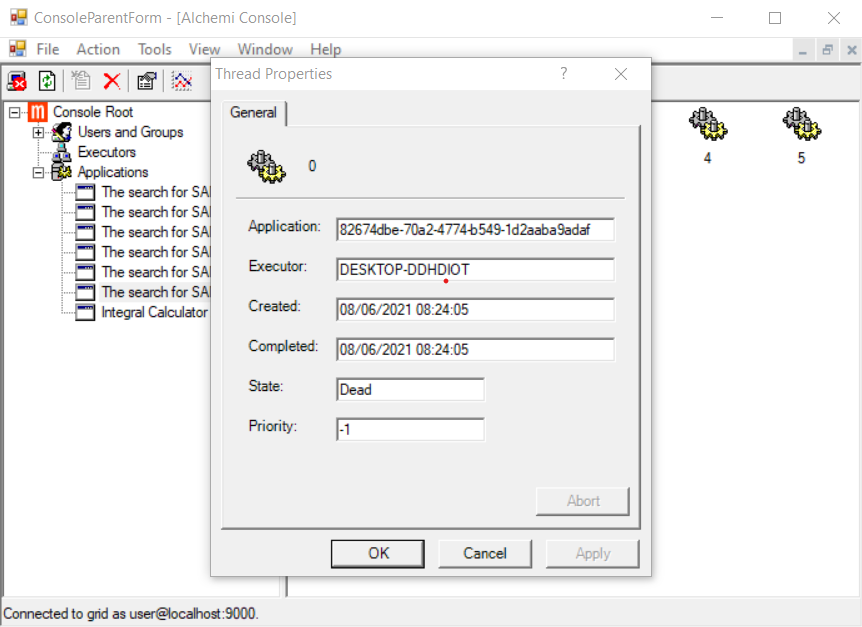
\includegraphics[scale=0.85]{1.0.png}
\end{center}



Hình 12: Luồng 1 do DESKTOP-TGSTI87 thực hiện
\begin{center}
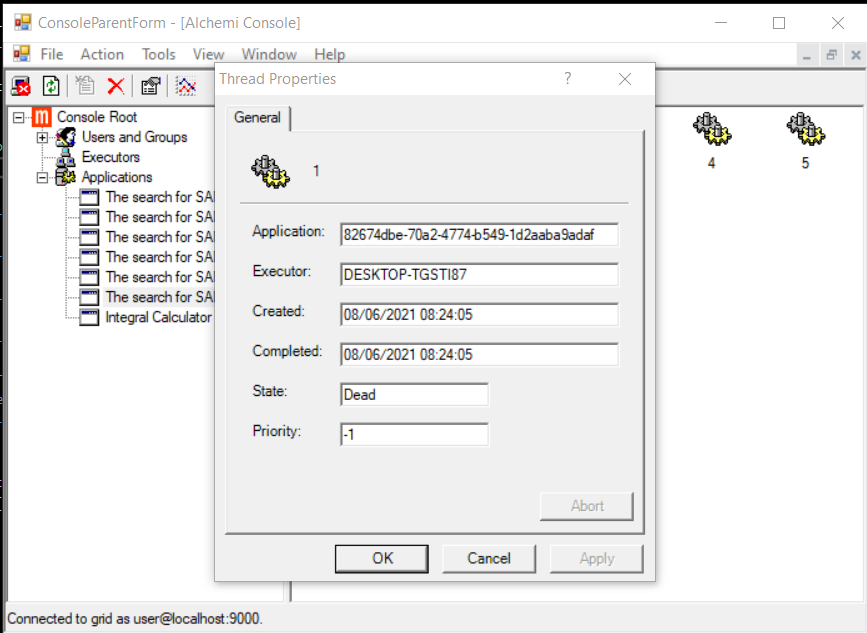
\includegraphics[scale=0.85]{1.1.png}
\end{center}





\end{document}